% Drawn by scripts/revision3/fig_appendix_schematics.py; the .pptx is the
% editable source and is released with the paper.
\begin{figure*}[t]
\centering
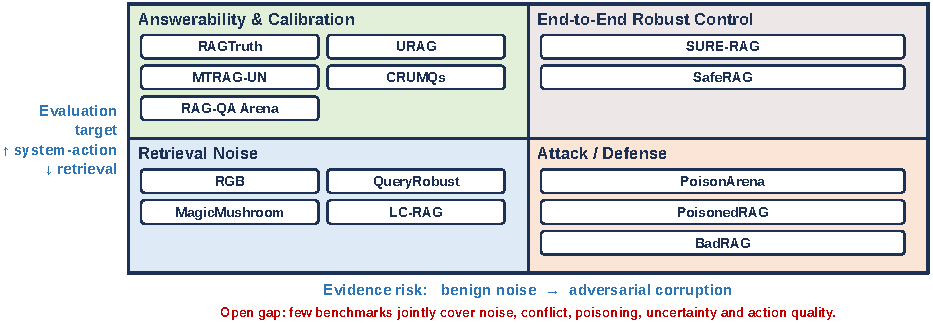
\includegraphics[width=\textwidth]{figures/generated/fig_benchmark_landscape.pdf}%
\caption{Conceptual benchmark landscape. Placement is illustrative rather than
data-derived; the figure organises differences in evidence risk and evaluation
level, not empirical distance or benchmark quality. The two axes are
coordinates C1 and C4, and the open gap is the reason a single ``robustness''
number rarely transfers between quadrants.}
\label{fig:benchmark-landscape}
\end{figure*}
